\documentclass[a4paper,12pt]{article} % класс документа
\usepackage[english, russian]{babel} % использование языковых вставок
\usepackage[T2A]{fontenc} % корректное ототбражение русских букв
\setcounter{tocdepth}{4} % подсчет в глубину вложений глав и секций
\setcounter{secnumdepth}{4} % аналогично предыдущему
\usepackage{xcolor} % использование цветовой граммы
\usepackage{hyperref} % использование гипертекста
\hypersetup{linkcolor=black, linkbordercolor=white} % настройка стиля гипертекста
\usepackage{bookmark} % использование отображения оглавленя в pdf приложениях
\usepackage{booktabs, float} % для форматирования таблиц
\usepackage{pgfplots} % для построения графиков
\pgfplotsset{compat = newest} % использование последней версии графопостроителя
\usepgfplotslibrary{fillbetween} % использование библиотеки для штриховки между графиками
\usetikzlibrary{patterns} % использование библиотеки шаблонов штриховки
\usepackage{indentfirst} % подключение библиотеки для красной строки
\usepackage{url} % для отображения url в списке литературы
\usepackage{pgfplots} % для построения графиков
\pgfplotsset{compat=1.9} % используется последняя версия построителя
\usepackage{graphicx} % для включения в работу построенных графиков
\graphicspath{ {./source/source_photos/} }

\newtheorem{theorem}{Теорема} % для определения теорем
\newtheorem{definition}{Определение} % для определения определений
\newcommand{\E}{\mathbb{E}}
\newcommand{\V}{\mathbb{V}}
\newcommand{\R}{\mathbb{R}}
\newcommand{\N}{\mathbb{N}}
\newcommand{\cov}{\text{cov} }
\newcommand{\myref}[1]{\ref{#1} стр. \pageref{#1}}

\AtBeginDocument{\renewcommand\contentsname{}}

\usepackage[14pt]{extsizes} % для того чтобы задать нестандартный 14-ый размер шрифта
\usepackage[utf8]{inputenc} % кодировка всего документа в UTF-8
\usepackage{amssymb, amsmath} %  математическое отображение символов
\usepackage[
	left=22mm, 
	top=20mm, 
	right=15mm, 
	bottom=20mm, 
	nohead,
	footskip=10mm
]{geometry} % настройки полей документа

\newcommand{\subsubsubsection}[1]{\paragraph{#1}\mbox{}} % для 4-ого уровня оглавления

\begin{document} 
	\setlength{\parindent}{1cm} % устанавливается красная строка размером в 1 cm.
	
	% Титульный лист
		% НАЧАЛО ТИТУЛЬНОГО ЛИСТА
\begin{center}
	\large{Московский Государственный Университет\\имени М.В. Ломоносова}\\
	\hfill \break
	\normalsize{\textbf{Экономический Факультет}}\\
	\hfill \break
	\normalsize{Кафедра Экономической Информатики}\\
	\hfill \break
	\hfill \break
	\hfill \break
	\hfill \break
	\large{Выпускная квалификационная работа по теме:}\\
	\hfill \break
	\large{\textbf{«Применение нейронных сетей и эконометрических методов} \textbf{в прогнозировании доходностей акций»}}\\
	\hfill \break
\end{center}
\hfill \break
\hfill \break
\hfill \break
\begin{flushright}
	\textbf{Выполнил:}\\
	Студент 4 курса э408 группы\\
	\hfill \break
	Гришин А. Ю.\\
	\hfill \break
	\textbf{Научный руководитель:}\\
	Кандидат экономических наук,\\
	Кандидат физико-математических наук,\\
	Кандидат юридических наук,\\
	Доцент кафедры Экономической Информатики\\
	\hfill \break
	Сидоренко В.Н.
\end{flushright}
\hfill \break
\hfill \break
\hfill \break
\hfill \break
\begin{center} Москва, 2023 \end{center}
\thispagestyle{empty} % выключаем отображение номера для этой страницы

% КОНЕЦ ТИТУЛЬНОГО ЛИСТА

	\newpage
	
	% Оглавление
	\tableofcontents
	\addcontentsline{toc}{section}{\LARGE Оглавление}
	\newpage
	
	\section{Введение} 
	Современный мир нельзя представить без валюты и денег в принципе. Каждый день всякий человек на Земле имеет с ними дело: кто-то с большей суммой, кто-то с меньшей, однако все мы неразрывно связаны с деньгами. Апогеем валютного триумфа в истории человека можно назвать создание предприятий: объединений людей на основе некоторой общей цели, которой впоследствии стали считать - получение прибыли. Логика проста: один человек получает сумму $N$ за один рабочий день $\Rightarrow$ 2 человек получат $2N$, однако, что даст им стимул к объединению усилий? Только факт того, что вместе они заработают $(2 + \varepsilon)N$ денег, где $\varepsilon$ - выигрыш от работы вместе. Но можно ли как-то получить сумму больше, чем указанная? Да, производить больше \footnote{Делай больше, клиент все купит - это очень похоже на тезис, что каждый товар находит своего покупателя $\Rightarrow$ тезис о "базаре справедливого обмена"\ Роберта Оуэна. Подробнее о том, что именно предлагалось сделать рассказано в работе \cite{ropert_ouwen}.} , пытаться подстраиваться под клиента \footnote{Человека/компании, который пользуется услугами данной компании.} : предугадывать потребности клиента и делать на конкретный товар скидку, пытаться угадать, когда спрос на тот или иной вид продукции будет больше в зависимости от времени года \footnote{Очевидно, что мороженое будут покупать заметно в меньших количествах зимой по сравнению с летом.}. То есть можно подстраиваться с двух сторон: работая над собой и изменять что-то внутри организации, а можно смотреть на то, что необходимо клиентам и делать именно это, именно тогда, когда это нужно. Получаются 2 крайности, которые необходимо уметь комбинировать. 
	
	Развивая финансовый рынок, получаем закономерное действие компаний --- выход на IPO \footnote{IPO - Initial Public Offering --- первый выход на биржу, когда компания продает свои акции неограниченному кругу лиц, делая их совладельцами.} и становление их публичными. Таким образом, уже владелец компании (он же владелец акции) стремится увеличить свою выгоду от владения долей, иначе зачем ему вообще тратить деньги на покупку ценных бумаг компании. Ведь важно то, чтобы вложенная сумма "отбивалась"\ с некоторой надбавкой, то есть человек зарабатывает то, что вложил, а также что-то сверх. Это сверх и есть искомый $\varepsilon$, который человек стремится увеличить как можно сильнее. Справедливо задать вопрос: "А зачем ему все это? Зачем вкладываться куда-то, чтобы получить больше?". Иными словами, зачем иметь больше того, чем есть сейчас? Логический ответ на это пытались дать многие экономисты, начиная с Адама Смита (1729–1737) \cite{adam_smith} и его идеей о рациональном человеке (homo economicus), однако большинство теорий, изложенных им же и позднее его последователями (членами классической школы) выдвигали это как предпосылку всего анализа. Следовательно, без выполнения данного условия о стремлении человека к максимизации собственной выгоды, большинство экономический теорий не являются работающими.
	
	Однако, опуская этот философский вопрос и возвращаясь к методам моделирования человеческого поведения, нельзя не заметить, что сами классики не углублялись в именно математическое моделирование и как следствие - описание экономической деятельности человека посредством формул, а делали это лишь через построения причинно-следственных связей, у истоков которых стояла проблема стоимости. 
	
	Намного позже Альфред Маршалл, английский экономист, живший в 1842-1924, являясь представителем неоклассической школы (кем его "обозвал"\ Торстейн Бунде Веблен), выпускает учебник "Принципы экономической науки"\ \cite{alfred_marshall}, в котором сводит воедино все труды и знания, полученные на пути развития и становления Экономики, а также собственные работы, посвященные применению наиболее полно описанного математического подхода к анализу экономической деятельности человека. 
	
	В настоящее время для анализа экономических показателей используются всевозможные методы будь то математические или нет. Однако Математика - точная наука, значит, если получится понять, когда и сколько продукции компании будет потреблять клиент (или получать дивидендов держатель акций), то можно будет без проблем еще сильнее уменьшить издержки на производство, что в свою очередь, приведет к получение еще большей экономической прибыли. 
	
	Так как в современной науке набирает популярность применение глубоких нейронных сетей к различным видам деятельности (медицина, металлургия, космическая промышленность, киноиндустрия, материаловедение, биология, биохимия, ...) \cite{nn_all_over_us}, значит, не лишнее - проверить, а имеет ли смысл вообще применять данные методы к финансовым задачам, а конкретно именно к предсказанию доходностей акций. 
	
	Настоящая работа является попыткой произвести сравнительный анализ наиболее популярных на данный момент математических моделей предсказания доходностей акций, примененных к 30 компаниям развитого (США) и развивающегося (Китай: Шанхай) рынков соответственно. Сравнение производится по характеристике качества прогнозирования доходности на 1 рабочий день биржи.
	\subsection{Актуальность}
		Данное исследование актуально с двух позиций: научная - выявив наиболее удачную с точки зрения предсказания на 1 день модель, в дальнейших исследованиях можно стараться развивать только ее, чтобы получать более точные результаты, а не пытаться выбрать между тем, над какой именно моделью из их множества работать, практическая - трейдерам или просто акционерам будет намного легче воспринимать временные ряды доходностей, так как они смогут с определенной точностью предсказывать конкретное значение подобного ряда на момент времени $t + 1$, что возможно даже приумножит их доход.
	\subsection{Цели}
		Целью настоящего исследования является помощь трейдерам или акционерам в прогнозировании доходностей акций. А умение качественно (с определенной точностью) предсказывать доходность приводит к умению формировать ответ на вопрос вида Buy or Hold? \footnote{Buy or Hold - Покупаем акцию или продаем?} достаточно быстро и аккуратно. Ведь основная проблема финансовых временных рядов - непредсказуемость, таким образом, нужно постараться решить данный вопрос так, чтобы на выходе было наиболее прибыльно и наименее рискованно, следовательно - наиболее точно. Отсюда появляется большая надежность финансовых инструментов с точки зрения человека, который заключает опционы или просто старается приумножить свое благосостояние посредством формирования собственного портфеля. Далее следует успешность фирмы, а отсюда, ведя разговор о финансовых рынках, возможность страны развить их еще сильнее и, возможно - увеличить благосостояние своих резидентов, а значит, возможность стать из развивающейся развитой. 
	\subsection{Задачи}
		Задачей текущего исследования является проведение сравнительного анализа между моделями машинного и глубокого обучения с целью выявления той, которая дает наиболее точный прогноз на период длиной 1 рабочий день биржи. Для этого: 1) Загружаем данные 2) Предобрабатываем данные 3) Проводим статистический анализ данных 4) Среди всех обученных алгоритмов выбираем тот, у кого лучший результат 5) Сформировать сравнительную таблицу между моделями по всем имеющимся данным. Несмотря на громоздкость поставленных задач, весь их комплект можно оформить в один алгоритм и, таким образом, применять его к любому набору входных данных (при условии, конечно, что входные данные - временной ряд). То есть появляется новая задача следующего вида: \textbf{на вход} программе подается временной ряд, \textbf{на выход} - показатели выбранной далее  тестовой статистики для каждой из рассматриваемых моделей. \footnote{Набор используемых моделей представлен в блоке ниже.}                  
	\section{Подготовительная часть}
	В чем заключается суть данной работы? С концептуальной стороны вопроса ответ очевиден: дан временной ряд, необходимо предсказать его следующее значение наиболее точным образом. Но прежде чем перейти к рассмотрению использованных моделей,  формализуем поставленную задачу, ведь не всегда понятно, что имеется в виду под "наиболее точно"\ и "временной ряд".
	\subsection{Формализация проблемы}
		Пусть на вход программе, назовем ее $f$, подается временной ряд вида: $y_t: t = \overline{1,N}$. Пока что никаких предпосылок относительно данного временного ряда нет. Тогда задача алгоритма $f$ предсказать $\hat{y}_{t + 1}$ так, чтобы значение $|\hat{y}_{t + 1} - y_{t + 1}|$ было минимальным. То есть $f: \mathbb{R}^{N \times 1} \to \mathbb{R} \Rightarrow f(y) = \hat{y}_{t + 1}, \text{где } y = \left(y_1,\ldots,y_N\right)^T$. В терминах глубокого обучения, имеем задачу класса sequence to one \footnote{Sequence to one - задача получения одного значения, исходя из набора данных. К таким задачам относят: семантический анализ текста, классификацию картинок и так далее.} . \textbf{Q}: Но в принципе, что такое временной ряд? \textbf{A}: Временной ряд - это последовательность значений, относящихся к одному объекту в разные моменты времени. То есть, за тот период, когда за объектом наблюдали и снимали показатели. В нашем случае временной ряд - это набор доходностей акций за определенный период времени, то есть не ставится ограничение на знак данных величин, ведь она (доходность) может быть как отрицательной, так и положительной. \textbf{Q}: Почему именно доходности? \textbf{A}: Говоря о них, нет необходимости задумываться о том, сколько реально стоит та или иная акция/ценная бумага: $20$ руб. или $2\text{'}000$ руб. В анализе доходностей нас интересует: насколько они изменяются относительно некоторого момента времени. \textbf{Q}: Какого момента? \textbf{A}: Логично представлять доходность как прирост вида:
		\begin{equation}
			r_{t} = \frac{y_{t} - y_{t - 1}}{y_{t - 1}} = \frac{y_{t}}{y_{t - 1}} - 1
		\end{equation}
		То есть, как изменяется в процентах цена на некоторый актив (не обязательно акцию, хотя в нашем случае именно на нее) относительно предыдущего рабочего дня биржи. Однако внутри самой "акции"\ фигурирует несколько показателей, характеризующих ее в конкретный момент времени: цена открытия, максимальная и минимальная цены, цена закрытия, скорректированная цена закрытия и общая сумма сделок. Акцент делается на анализе цен открытия (так как с точки зрения автора работы важнее всего - хорошо начать рабочий день), хотя несомненно наличие взаимосвязи между ценой открытия и закрытия или иными доступными показателями. Когда есть возможность - другие показатели включаются в анализ, когда нет такой возможности (классическая модель не предназначена) - не включаются. Подводя итог: \textbf{Дано}: $y = \left(y_1, \ldots, y_n\right)^T$, \textbf{Найти}: $\hat{y}_{N + 1}: |\hat{y}_{N + 1} - y_{N + 1}| \to \min$. Подставляя вышеупомянутое равенство, имеем задачу оптимизации:
		\begin{equation}
			|f(y) - y_{N + 1}| \to \min_{\beta \in \mathbb{R}^k}
		\end{equation}
		Где $\beta$ - набор параметров модели, хотя некоторые из них имеют неоптимизируемые параметры (гиперпараметры), но в общем случае задача имеет подобный вид. Но проблема в том, что $y_{N + 1}$ неизвестно, а значит, невозможно подобрать алгоритм абсолютно точного прогнозирования, значит, необходимо на основе имеющейся информации сформировать алгоритм, который наиболее точным образом описывает предложенные ему данные, а далее делает предсказание, причем предсказание, как можно меньше отличающееся от реального значения. Только теперь, проведя подобные рассуждения, мы находимся в области машинного обучения и можем говорить о гипотезах рынка \footnote{Гипотезы рынка - обоснование исследования на качественном уровне, то есть утверждения о возможности проводить какой-либо технический анализ.} . Ведь для каждого типа рынка характерны свои особенности, следовательно, закономерный вопрос: почему мы вообще имеем право пытаться предсказывать что-то для развитой или развивающейся экономик. Изложение двух нижестоящих теорий представлено в сжатом виде, что делает повествование о них поверхностным, но достаточным для понимания всех особенностей работы.
		\subsubsection{Гипотеза эффективного рынка}
			Это одна из самых неоднозначных в плане количества последователей инвестиционная теория, ставящая своей целью описать принципы движения цен на активы, первоначальная версия которой "представлена"\ Луи Башелье в 1900 году. В его работе показана независимость доходности акций от течения времени, таким образом, Башелье пришел к выводу: "Вероятность роста цены в любой момент времени равна вероятности ее падения, а математическое ожидание спекулянта равно нулю". Много раз менявшая свою формулировку, начиная с Пола Самуэльсона: "На конкурентных рынках на всякого продавца найдется покупатель. Если можно быть уверенным, что цена вырастет, значит, она уже выросла"\ ,  в 1960-ых годах она (гипотеза) приобрела формальный вид в труде Юджина Фамы, использовавшего в исследованиях модель случайного блуждания, выведенную Башелье. По итогам эксперимента, Юджин Фама \cite{efficient_market} привел доказательство того, что вся доступная информация уже заложена в бумагах (позднее: "рынок полностью отражает всю доступную информацию"), то есть бесполезно пытаться предугадывать цены, любое предсказание не сбудется. Более того, единственный фактор, который способен повлиять на цену - это выходящие в будущем новости. А значит, перманентное доминирование над рынком не является возможным, а активное инвестирование не является состоятельным. Более подробная информация изложена в статье от 13 сентября 2022 года \cite{fama_market_efficiency}. На данный момент существует 3 основных гипотезы эффективности рынка:
			\begin{enumerate}
				\item \textbf{Слабая гипотеза} - в цене содержится вся историческая информация об активе и только фундаментальный анализ иногда может обеспечить избыточную доходность.
				\item \textbf{Полусильная гипотеза} - в ценах содержится вся публичная информация, таким образом, избыточную доходность может обеспечить только закрытая от широкой публики информация (инсайдерская).
				\item \textbf{Сильная гипотеза} - в ценах содержится как общедоступная, так и закрытая информация. Таким образом, ничто не может дать инвесторам избыточную доходность по сравнению со среднерыночным показателем.
			\end{enumerate}
			Тогда напрашивается вывод: если быть сторонником ГЭР, то настоящая работа не имеет смысла, ведь технический анализ не может дать дополнительной доходности для любой степени ее силы. Однако, по словам Мартина Свэлла, проанализировавшего историю данной гипотезы в работе \cite{matrin_swell}: "Строго говоря, гипотеза [прежде всего, в ее сильной форме] ложна, но по духу глубоко верна $\ldots$ До тех пор, пока текущая гипотеза не будет заменена лучшей гипотезой, критика имеет ограниченную ценность". Отсюда все-таки следует обоснование, почему существует так много математических моделей, пытающихся прогнозировать доходность активов. Отсюда следует, что в современном мире количество методов предсказания настолько велико, что исследователю сложно выбрать нужный, это еще одно подтверждение, почему настоящая работа имеет смысл.
		\subsubsection{Гипотеза фрактального рынка}
			Часто в качестве доказательства ложности ГЭР приводятся в пример финансовые кризисы, так как по ГЭР вероятность возникновения подобного кризиса пренебрежимо мала или приблизительно ноль. Таким образом, появляется еще одна гипотеза: Гипотеза Фрактального Рынка (ГФР), чьим родоначальником является Бенуа Мандельброт \cite{benoit_mandelbrot}, по которой можно объяснять кризисы. Ее основные характеристики: 1) график доходностей активов имеет фрактальную (всегда $1 < D <2$) размерность 2) Различные окна (интервалы) исходного графика могут быть самоподобными 3) Каждому финансовому графику присуща своя уникальная структура и соответственно ее свойства 4) Финансовый график обладает памятью о своих исходных условиях (имеет долгосрочную память; формальный способ проверки данного утверждения вводится позже). Для выполнения данной гипотезы предполагается, что рынок является стабильным, если он включает в себе очень много инвесторов с различными горизонтами планирования (это гарантия ликвидности). Объяснение кризисов происходит следующим образом, описанным в статье Палювиной А.С. \cite{fractal_market}: "Когда инвесторы меняют свои инвестиционные горизонты (например, фундаментальная информация становится ненадёжной, а	долгосрочные инвесторы уходят с рынка или сокращают свои горизонты),	баланс между краткосрочной и долгосрочной перспективами искажается,	рынок становится менее ликвидным и возникает кризис". Таким образом, из данной гипотезы следует вывод, что информационный и инвестиционный горизонты оказывают влияние на поведение инвестора.
		\subsubsection[Проверяемая гипотеза]{Проверяемая гипотеза настоящего исследования}
			Гипотеза, подтверждение которой настоящая работа ставит одной из своих ключевых задач, заключается в проверке суждения, что нейросетевой (далее NN) поход является наиболее эффективным применительно к исследуемой области финансовых рынков, а точнее к временным рядам цен/доходностей акций. То есть главный вопрос: нейросеть лучше справляется с прогнозированием доходностей акций по цене открытия на один рабочий день биржи по сравнению с другими использованными моделями или нет?
	\subsection{Наиболее популярные методы решения}
		
		\subsubsection{Exponentially Weighted Moving Average}
		\subsubsection{Auto-regressive Integrated Moving Average}
		\subsubsection{Generalized Auto-Regressive Conditional Heteroskedasticity}
		\subsubsection{Auto-regressive Fractionally Integrated Moving Average}
		\subsubsection{Fractionally Integrated GARCH}
		\subsubsection{Self Exciting Threshold Auto-regressive Moving Average}
		\subsubsection{Neural Network}
		\subsubsection{Singular Spectrum Analysis}
		\subsubsection{Transformers и моделирование сезонности}

	\section{Описание данных и эксперимент}
	\subsection{Развивающийся рынок (Китай)}
	\subsection{Развитый рынок (США)}
	\section{Обсуждение выводов}
По результатам эксперимента настоящего исследования сформирована итоговая сравнительна таблица ранее отобранных моделей. Сравнение производится как для развитых, так и для развивающихся рынков. Оценка модели происходит на основе ее способностей прогнозировать как цены, так и доходности на 1 рабочий день биржи.

Однако, исходя из имеющегося количества данных, а именно $15 \cdot 2 \cdot  2 \cdot 15 = 900$ значений, для удобства визуального восприятия производим дробление вида: компания; модель; ошибка. Подобная структура имеется как для доходностей и цен, так и для рынков Китая и США. Для начала смотрим на полученные результаты относительно цен на развитом рынке. После этого переключаемся на доходности. Далее аналогичным образом проходимся по развивающемуся рынку.

Подобный план представления полученного результата сформирован для более удобного восприятия читателем, так как большое количество данных почти всегда равно трудностям в понимании выводов.

\begin{figure}[H]
	\centering
	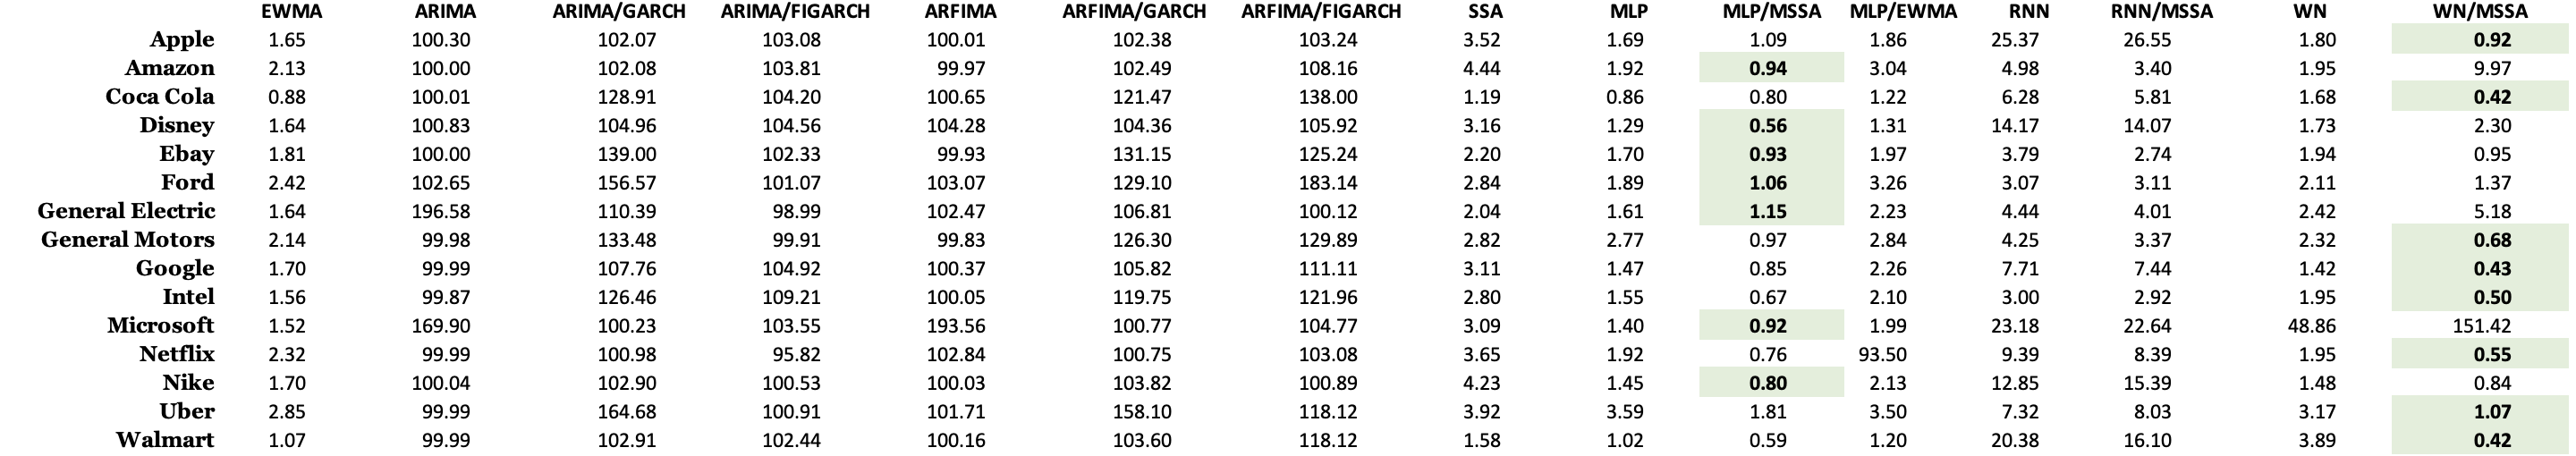
\includegraphics[width= 17cm]{./final tables/us_prices.png}
	\caption{Таблица итоговых значений WAPE (США, цены) в \%}
	\label{pic::final_table_us_prices}
\end{figure}

\noindent Исходя из полученных данных, видим, что в основном соревнование ведется между моделями Multilayer Perceptron (\myref{link::neural_networks}) в комбинации с отчисткой данных от шума посредством Multistage Singular Spectrum Analysis (\myref{link::mssa}) и Wavelet Network (\myref{link::wavelet_nets}). Интересно, что для большинства рассмотренных компаний WN + MSSA дает более точный прогноз на 1 рабочий день биржи, что наталкивает на гипотезу о превалировании или простом наличии доминантных частот в ценах на развитом рынке. Это и позволяет самообучающейся функции <<подгоняться>> (обучаться) именно на них, что дает частотно-временному анализу преимущество перед классическим подходом MLP. Данный вопрос достаточно интересен и требует более детального анализа, который производится в последующих работах автора настоящего исследования. Однако нельзя забывать и об успехах MLP + MSSA, ведь именно данная модель занимает второе место в прогнозе цен. В средних же величинах --- посредством усреднения для всех компаний --- у MLP + MSSA показатель WAPE равняется $1.08\%$, а у WM + MSSA $11.8\%$, что безусловно выводит MLP + MSSA на 1-ое место. Однако, вычислив средние по выделенным зеленым значениям, получаем WN + MSSA ($0.62\%$), а MLP + MSSA ($0.91\%$), что делает частотно-временную модель более точной в прогнозах. Отсюда нельзя сделать однозначный вывод о победе той или иной модели, так как они <<идут бок о бок>>, следовательно, необходимо в процессе построения прогнозного значения опираться на результат каждой из них. То есть для прогноза цен открытия рассмотренных компаний выявлены два победителя: MLP + MSSA и WN + MSSA.

Нельзя не заметить результаты статистических моделей --- ничего не думающих об имеющихся данных --- EWMA (\myref{link::ewma}) и SSA (\myref{link::ssa}). Данные модели не делают никаких предпосылок относительно анализируемых данных, однако ошибки их прогнозов не так далеки от лидеров данной гонки. Это наталкивает на мысль о возможном компромиссе относительно применяемой модели: если нужно максимальное качество (и при этом есть время), то WN + MSSA или MLP + MSSA, иначе (если необходим максимально быстрый ответ) EWMA или SSA. Рассмотренные только что 4 модели выделяют наиболее выдающиеся результаты, полученные, исходя из имеющихся данных. Другими словами, нельзя однозначно говорить о $100\%$-ой гарантии наличия доминантных частот в сигнале без дополнительного исследования. Но можно сформулировать гипотезу об этом. Также нельзя утверждать, что для остальных компаний этих же рынков результат будет аналогичным, так как все компании индивидуальны. Значит, \textit{основываясь на имеющихся данных рассмотренных компаний}, получаем максимальную точность у WN + MSSA и MLP + MSSA для развитого рынка. Далее идут EWMA и SSA.

Глядя на все эконометрические модели, видим, что их средняя ошибка для рассмотренных компаний составляем $112.07\%$, а фактические величины WAPE почти не опускается ниже $100\%$, что делает проанализированные модели практические непригодными для работы с финансовыми рядами рассмотренного типа (цены открытия). Однако лучшими моделями в данном блоке являются ARIMA и ARFIMA, дающие результат в среднем $100\%$ отклонение.

Относительно рекуррентных моделей типа RNN, RNN + MSSA нельзя сказать, что они совершенно непригодны для работы с временными рядами, однако, основываясь на \cite{transformers_are_useless_for_TSF}, видим, что все-таки временные ряды не то, где подобного рода модели имеют большое преимущество. Как уже говорилось ранее для успешной работы рекуррентной сети необходима задача обработка естественного языка, то есть --- набора слов/предложений, а не просто чисел, как в случае с анализом временных рядом, так как в тексте есть смысл, который и пытается <<вытащить>> модель.

Переходя к анализу доходностей для развитого рынка, сморим на полученную таблицу значений. Видим безоговорочную победу модели RNN + MSSA, что объясняется успешной очисткой данных от шума и последующим извлечением некоторого смысла из него посредством алгоритма RNN. Остальные модели --- все, кроме RNN --- показывают плохой результат, близкий к значениям эконометрических моделей на ценах развитого рынка. Из этого делаем вывод, что для рассмотренного набора доходностей имеющихся компаний почти одинаково плохо подходят как эконометрические, так и нейросетевые модели. Победителем в этой <<гонке>> является RNN + MSSA, однако нельзя забывать о примерах работы данной модели (\myref{link::rnn_module}), когде отчетливо показывается неспособность RNN семейства достаточно точно \footnote{Под словом <<точно>> имеется формирование среднего меньше, чем отклонение. Данное дополнение к имеющейся обученной модели позволяет достоверно оценивать финансовые риски.} предсказывать доходности. Таким образом, формально лидер определен, но подобный результат, им предоставляемый, не является валидным для практического применения и требует более тщательного анализа.
\begin{figure}[H]
	\centering
	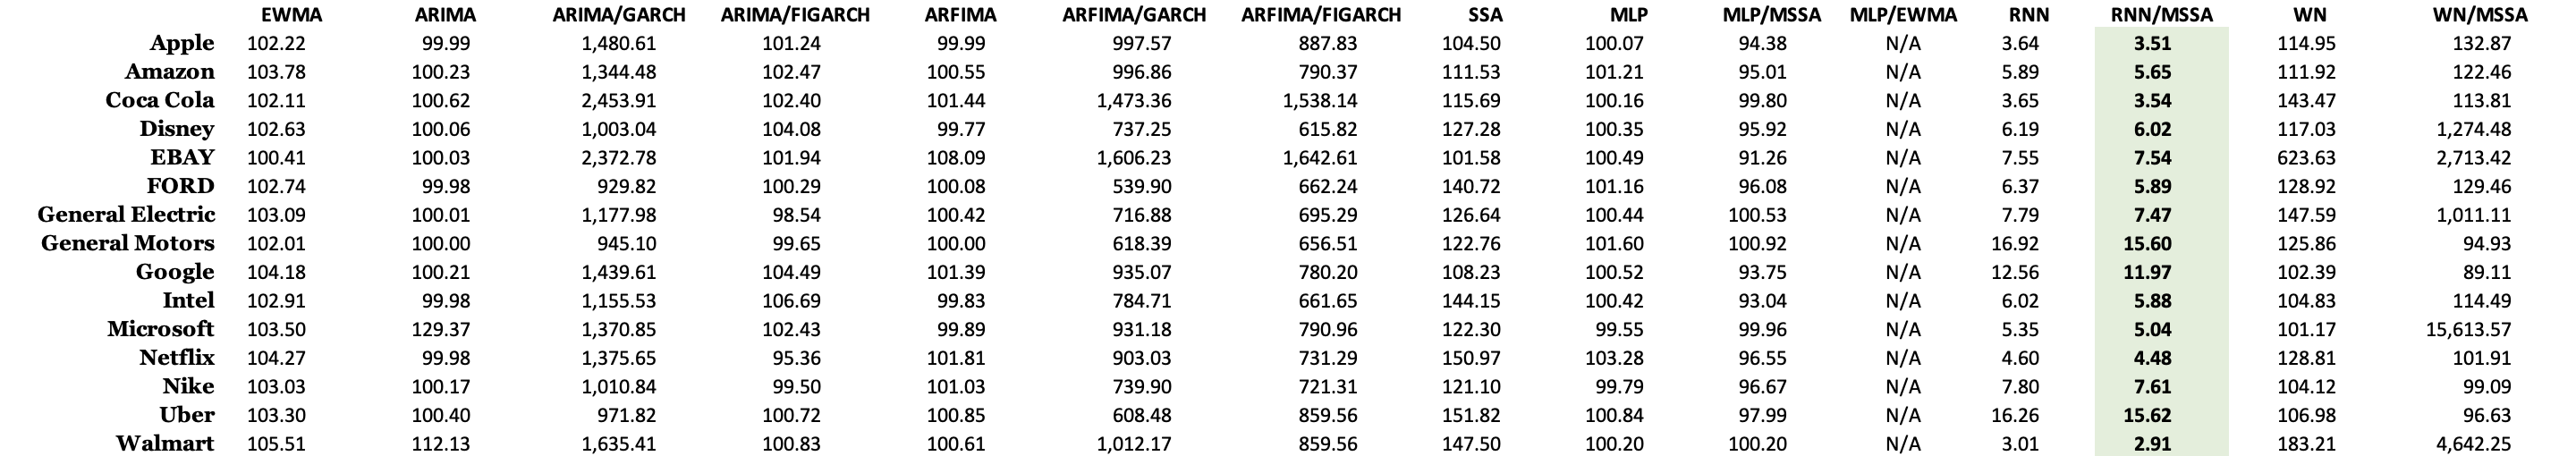
\includegraphics[width= 17cm]{./final tables/us_returns.png}
	\caption{Таблица итоговых значений WAPE (США, доходности) в \%}
	\label{pic::final_table_us_returns}
\end{figure}

\noindent Блок MLP + EWMA для доходностей не заполнялся, так как вычисление экспоненциального сглаживания доходностей для автора исследования не носит как практического, так и экономического смысла.

\begin{figure}[H]
	\centering
	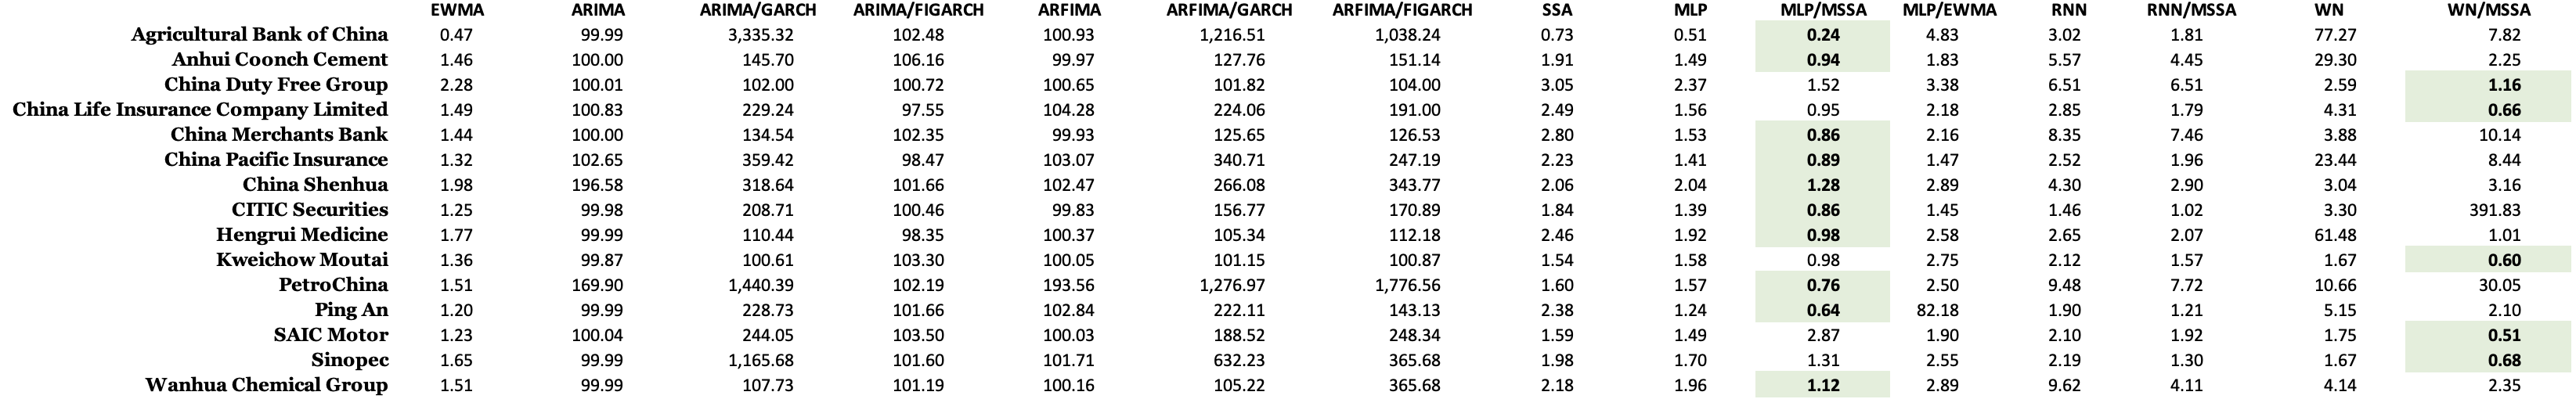
\includegraphics[width= 17cm]{./final tables/china_prices.png}
	\caption{Таблица итоговых значений WAPE (Китай, цены) в \%}
	\label{pic::final_table_china_prices}
\end{figure}


Переходим к блоку развивающегося рынка и аналогичным образом смотрим на показатели WAPE для цен. Ситуация очень похожа на только что рассмотренный развитый рынок: WN + MSSA и MLP + MSSA конкурируют друг с другом. Однако тут первенство все-таки остается за MLP + MSSA с достаточно большим перевесом. Среднее значение для MLP + MSSA равно $0.86\%$ (для выделенных зеленым цветом), а для WN + MSSA --- $0.72\%$, что аналогично показывает более точные прогнозы у WN + MSSA, однако уже на меньшем количестве компаний. Лидером соответственно становится MLP + MSSA (с оговоркой на наличие WN + MSSA, который старается дотянуться до своего оппонента).

Статистические модели аналогично показывают сравнимый с MLP + MSSA результат, не выдавая при этом каких-либо кардинальных различий между своей работой на развитом и развивающемся рынках. Это говорит об их стабильности (инвариантности) относительно самого поведения анализируемых величин.

Эконометрические модели в свою очередь в среднем дают $263.43\%$ отклонение, что делает их еще более непригодными моделирования временных рядов рассмотренных компаний. Однако лучшими на данный момент являются ARIMA + FIGARCH и ARFIMA, дающие в среднем $104.38\%$-ое отклонение. В любом случае, данные модели не применимы к реальной жизни из-за слишком большой ошибки.

Ситуация с применением алгоритма MSSA остается аналогичной, так как очистка рассмотренных данных дает прирост к качеству прогноза той или иной модели. Соответственно алгоритм MSSA в среднем (тут важно помнить о комбинации WN и MSSA) дает более хороший результат, что привлекает более пристальное внимание к принципу его работы \cite{kuang2020efficient}. 

\noindent Далее смотрим на полученные результаты для доходностей на развивающемся рынке:

\begin{figure}[H]
	\centering
	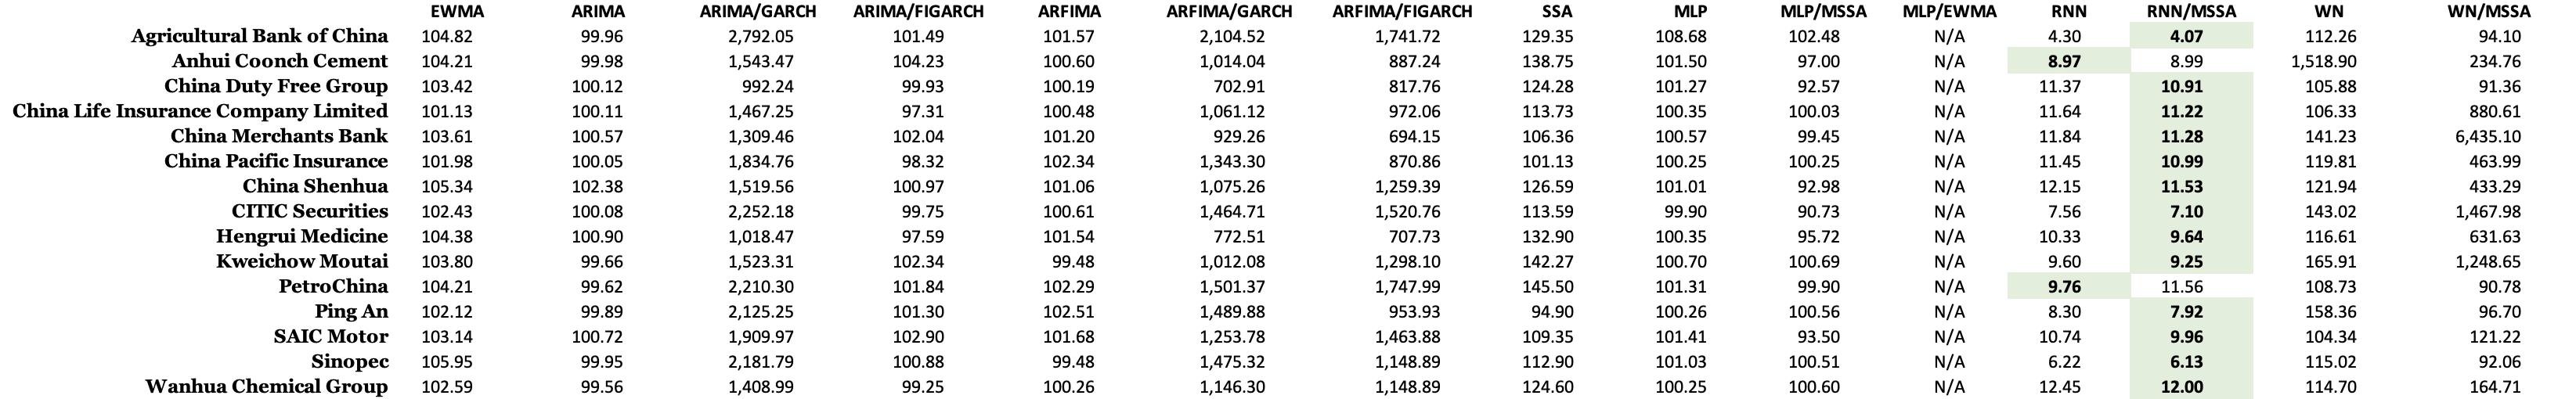
\includegraphics[width= 17cm]{./final tables/china_returns.png}
	\caption{Таблица итоговых значений WAPE (Китай, доходности) в \%}
	\label{pic::final_table_china_returns}
\end{figure}

\noindent Как и ожидалось результат повторяется, то есть RNN + MSSA показывают лучшие значения для всех имеющихся моделей. Исключением при этом являются компаниии Anhui Coonch Cement и Kweichow Moutai, для которых RNN дает результат лучше, чем RNN + MSSA. Это пример того, что алгоритм MSSA не является универсальным средством и может давать не только улучшение, но и ухудшение посредством случайного удаления информации о важных показателях сигнала, содержащих тренд. Все остальные модели аналогичным образом показывают результат около или даже выше $100\%$-ого отклонения, что автоматические делает их неприменимыми к реальности.

Подводя итог блоку анализа результатов, выделяем несколько наиболее важных вещей, сформулированных в ходе эксперимента: 1) WAPE для прогнозов цен заметно меньше почти для всех (за исключением эконометрических) моделей, чем WAPE для доходностей. То есть для имеющихся данных проще предсказывать именно цены 2) MSSA + MLP, а также MSSA + WN являются лидерами в области прогнозирования цен для проанализированных компаний 3) MSSA + RNN является лучшей для предсказания доходностей, однако ее результаты не являются допустимыми для применения к реальности в силу достаточно большой ошибки относительно сравнительно малого среднего значения прогноза 4) Эконометрические модели плохи как для прогнозов цен, так и для прогнозов доходностей (опять же вывод происходит из имеющихся данных и не носит $100\%$-ый характер) 5) Алгоритма очистки от шума MSSA показывает отличный результат, добавляя почти ко всем моделям в точности прогноза как цен, так и доходностей. Исключением тут модель WN + MSSA. Факт успешного применения MSSA объясняется наличием большого количества шума в имеющихся данных. То есть моделям лучше <<настраиваться>> на чистые значения того или иного показателя, в нашей терминологии --- тренд.

Дополнением к данному блоку служит формулировка гипотезы, проверяемой автором в будущих исследованиях:
\begin{uncertainty}
	Для цен активов развитого финансового рынка характерно наличие большего количества частотных составляющих, чем для развивающегося.
\end{uncertainty}

	\section{Заключение}
	
	% Список литературы
	\newpage
	\bibliographystyle{plain}
	\bibliography{./source/bibliography/bibliography}
	\addcontentsline{toc}{section}{Список литературы}
\end{document} 